\documentclass{article}

% if you need to pass options to natbib, use, e.g.:
%     \PassOptionsToPackage{numbers, compress}{natbib}
% before loading neurips_2018

% ready for submission
% \usepackage{neurips_2018}

% to compile a preprint version, e.g., for submission to arXiv, add add the
% [preprint] option:
%     \usepackage[preprint]{neurips_2018}

% to compile a camera-ready version, add the [final] option, e.g.:
     \usepackage[final]{nips_2018}

% to avoid loading the natbib package, add option nonatbib:
%     \usepackage[nonatbib]{neurips_2018}

\usepackage[utf8]{inputenc} % allow utf-8 input
\usepackage[T1]{fontenc}    % use 8-bit T1 fonts
\usepackage{hyperref}       % hyperlinks
\usepackage{url}            % simple URL typesetting
\usepackage{booktabs}       % professional-quality tables
\usepackage{amsfonts}       % blackboard math symbols
\usepackage{nicefrac}       % compact symbols for 1/2, etc.
\usepackage{microtype}      % microtypography
\usepackage{graphicx}
\usepackage{subcaption}
\usepackage{amsmath}
\usepackage{multirow} 


\graphicspath{ {imgs/} }

\title{Transfer Learning Approach for Processing Extreme Low-Light Images}

% The \author macro works with any number of authors. There are two commands
% used to separate the names and addresses of multiple authors: \And and \AND.
%
% Using \And between authors leaves it to LaTeX to determine where to break the
% lines. Using \AND forces a line break at that point. So, if LaTeX puts 3 of 4
% authors names on the first line, and the last on the second line, try using
% \AND instead of \And before the third author name.

\author{%
  Nalin Gupta \\
  \texttt{NUID: 001497315} \\
  \And
  Christopher Botica\\
  \texttt{NUID: 001726854} \\
  \And
  Tyler Brown\\
  \texttt{NUID: 001684955} \\
  % Coauthor \\
  % Affiliation \\
  % Address \\
  % \texttt{email} \\
  % \AND
  % Coauthor \\
  % Affiliation \\
  % Address \\
  % \texttt{email} \\
  % \And
  % Coauthor \\
  % Affiliation \\
  % Address \\
  % \texttt{email} \\
  % \And
  % Coauthor \\
  % Affiliation \\
  % Address \\
  % \texttt{email} \\
}

\begin{document}
% \nipsfinalcopy is no longer used

\maketitle

\section{Introduction}

Images taken in low-light conditions are often too dark, noisy, and
distorted to be used in industrial purposes. We propose a deep-learning model that processes low-light images to improve image brightness and increase their overall quality \footnote{https://github.com/tbonza/CS7180}. The problem with imaging in low-light conditions is challenging due to low-photon count and low Signal-to-Noise (SNR) ratio. This yields very dark and noisy images. The most common techniques to overcome this problem are long exposure shot and increased ISO However, the first method assumes a static scene and yields blurry images with the slightest camera shake. Additionally, increasing the ISO, or, in other words, allowing more light to enter the camera in a short amount of time, increases the amount of noise \cite{chen2018learning}. Thus, common post-processing techniques brighten the image at the expense of image quality. Being able to ``see in the dark'' provides a number of real-world benefits such as photography, computer vision, and social networking. 

By introducing our transfer learning-based model for extreme low-light image processing, we contribute to the advancement of this field with the following:

%
%....
%Success of data simulation and transfer learning model
%....
%Showed improvement with 10\% training data
%....
%Proof of concept: generalize to other domains/devices where %data is expensive, such as Medical Image data, UAV, Autonomous %Cars, etc.
%

\begin{itemize}
    \item Novel technique for simulating low light images.
    \item Reduced cost of data collection due to improvements on data augmentation of publicly available datasets such as RAISE 6k or ImageNet.
    \item Proof of concept for zero-shot and transfer learning using augmented data to predict on naturally dark images with only 10\% of data used by Chen et. al. (2018) \cite{chen2018learning}. This can be generalized to other domains with scarce training data such as medical imaging and autonomous driving. 
\end{itemize}

\section{Related Work}

In the past, the problem of enhancing low light images has been tackled via noise reduction. This noise becomes dominant especially in low-light images due to low SNR. Remez et. al. proposed a deep CNN for noise reduction under
the assumption that this low-light noise belongs to a Poisson
distribution \cite{remez2017deep}.  The team used images from ImageNet as their ground truth data
and added synthetic Poisson noise to simulate corrupted images \cite{imagenet_cvpr09}. Even though
their model outperforms the state-of-the-art denoiser ``BM3D'', it does not
scale well to real-world images, since their dark image simulation does not capture the true distortions of low-light images.
Furthermore, their model only denoises images but does not brighten them.


Motivated by these downfalls, Chen et. al., proposed an end-to-end CNN,
``See-in-the-Dark'' (SID), which brightens extremely low light images and
removes noise without making any underlying assumptions
\cite{chen2018learning}. However, these advances come with the added expense
of collecting large amounts of low
light and bright light images. In the absence of a true vs noisy image
dataset, this team captured scenes using various exposure times to generate
true (bright light) and corrupted (low light) image pairs called
``See-in-the-Dark Dataset'' (SID Dataset
\footnote{https://github.com/cchen156/Learning-to-See-in-the-Dark}). However,
their model is built only for raw images, is camera specific, and not easy to generalize.\newline

We propose a transferable CNN for image brightening and denoising. Instead of training our model on actual true (bright light) and corrupted (low light) image pairs, we use the high-resolution images from the publicly available RAISE-6k raw image dataset \cite{Dang-Nguyen:2015:RRI:2713168.2713194}. We use these as our true images and corrupt these by simulating low-light conditions for use in our model. We train our CNN on this synthetic data to obtain our initial model parameters. A small fraction of the real images paired from the SID dataset is then used in our transfer learning \cite{Goodfellow-et-al-2016} approach to update our model parameters. These model parameters are updated for the particular camera used in the SID dataset. We then use this model to test on the SID Dataset. In addition, we aim to test various transfer learning approaches, such as traditional transfer learning and zero shot learning \cite{larochelle2008, NIPS2009_3650,socher2013zeroshot}. 

The novelty of our approach stems from the idea of ``more for less''. Our
model drastically reduces the overhead costs of data collection by
synthesizing readily available training data (RAISE-6k raw images dataset).
This is particularly beneficial in domains where images pair collection is
expensive/time-consuming.

\section{Methods}

We collect 6000 images from the publicly available dataset RAISE-6k to simulate extreme low-light conditions and train our first model. RAISE-6k is the largest collection of publicly available high-resolution images (> 2000x4000 pixels). However, these images, along with the images from the SID dataset, are in raw format. Therefore, as a precursor to our simulation and testing, we transform all these images into standard RGB format. 

We first simulate extreme low-light images from RAISE-6k, train our model on these simulated images, and then transfer our model to train on a fraction of the true dark vs bright images from the SID dataset.

\begin{figure}[t!]
  \centering
  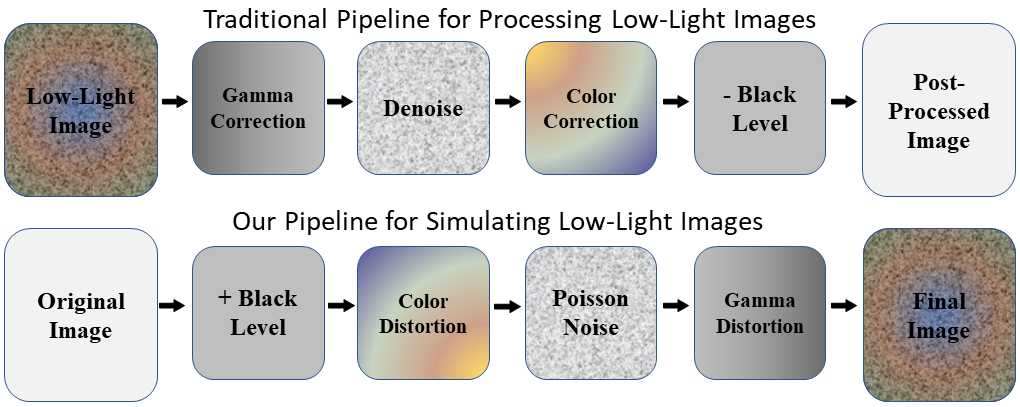
\includegraphics[scale=0.35]{simulation_flowchart}
  \caption{\textbf{Top:} Traditional pipeline for processing low-light images,            \textbf{Bottom:} Our pipeline to simulate low-light images (reverse of traditional pipeline)}
  \label{fig: simulation pipeline}
\end{figure}

\subsection{Simulating Low Light Images}
As illustrated in Figure \ref{fig: simulation pipeline}, a traditional image processing pipeline takes a corrupted/low-light image and applies the following sequence of modules: gamma correction, denoising, color correction, and black level reduction to provide a processed denoised image. We use this information to synthetically generate low-light images by applying the reverse of this pipeline on bright images. 

For a given bright image, $B_{m\times n\times 3}$ and corresponding low-light image, $D_{m\times n \times 3}$, where each pixel of the bright image, $b_{i, j, k}$ and low-light image, $d_{i, j, k}$ is an integer value $\in [0, 255]$ we want to approximate the parameters $bl$, $w_r$, $w_g$, $w_b$, $\gamma$ of a function $f$ such that, 
$$f(B_{m\times n\times 3} |\; bl, w_r, w_g, w_b, \gamma) \approx D_{m\times n\times 3}$$
Here $f(\bullet)$ is the composite function comprising of each module as shown in the bottom part of Figure \ref{fig: simulation pipeline} and $bl$, $w_r$, $w_g$, $w_b$, $\gamma$ correspond to the parameters associates with black level, color distortion (for color channels red, green and blue), and gamma respectively. Our initial approach to creating simulated low light images was to randomly select values for \(\gamma, w_{R}, w_{G}, w_{B},\) and \(bl\) and validate them by visualizing the distorted image. However, this process is not sufficient to yield accurate results. This lead us to use 200 image pairs from the SID dataset to approximate the parameters of the black level, color distortion and gamma modules. Since the input to the Poisson noise generator is the image itself, we do not need to approximate a parameter for this process \cite{remez2017deep}. A description of each module is provided below. 

\subsubsection{Black Level}
The black level function, $BL(\bullet)$, is defines as, 
$$BL(B_{m\times n\times 3}) = max(B_{m\times n\times 3} - bl,\;0) \text{, where }  bl \in [0, 255]$$
This function reduces the overall brightness of the image and brings it closer to the dark image. We approximated the value of $bl$ for a image pair by taking the average difference between their corresponding pixel values, 
$$bl = \frac{1}{3mn}\sum{(b_{i, j, k} - d_{i, j, k})} \; \;\; b_{i, j, k} \in B_{m\times n\times 3},\;\; d_{i, j, k} \in D_{m\times n\times 3}$$
The distribution for the $bl$ values obtained from the image pairs is shown in Figure \ref{fig:simulation variables}(a).

\subsubsection{Color Distortion}
The color distortion function uses parameters, \(w_r, w_g,\) and \(w_b\) which correspond to weights for the Red, Green, and Blue color channels of the image. The color distortion function, $CD(\bullet)$, is defined as, 
$$CD(B_{m\times n\times 3}) = [w_r, w_g, w_b] \cdot B_{m\times n\times 3}$$
where each weight \(w_r, w_g,\) and \(w_b\) is multiplied by its corresponding color channel in the bright image. The color distortion aims to reduce the intensity of each color non-uniformly, while distorting the color space, to simulate low-light conditions. We approximate \(w_r, w_g,\) and \(w_b\)  for a image pair by taking the average ratio between their corresponding pixels (for each channel), 
$$w_a = \frac{1}{3mn}\sum{(\frac{d_{i, j, a}}{b_{i, j, a}})} \text{, where }b_{i, j, k} \in B_{m\times n\times 3},\;\; d_{i, j, k} \in D_{m\times n\times 3}, \;\; a \in [r,\; g,\; b]$$
The distribution for the \(w_r, w_g,\) and \(w_b\) values for each color channel is shown in Figure \ref{fig:simulation variables}(b). 

\begin{figure}[t!]
  \centering
  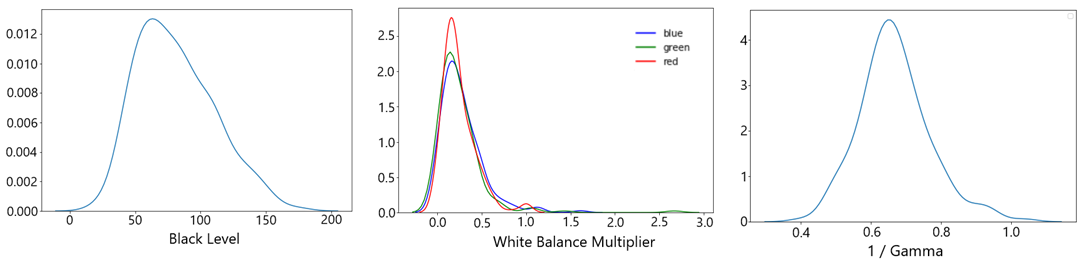
\includegraphics[scale=0.5]{Distributions}
  \caption{Approximated parameter value distributions for (a) Black Level, (b) Color Distortion, and (c) Gamma Correction. We use these to generate a multinomial distribution and sample from it to obtain our parameters. These parameters are used to generate low-light images.}
  \label{fig:simulation variables}
\end{figure}

\subsubsection{Noise}
According to \textit{Remez et. al.} \cite{remez2017deep} low-light inherently have Poisson noise. For the Poisson noise function, $PN(\bullet)$, we simply add Poisson noise to our images to simulate low-light conditions:
$$PN(B_{m\times n\times 3}) = poisson(B_{m\times n\times 3}/255)*255$$
Note that the input to the Poisson distribution is in the interval \([0, 1]\). Therefore, we first scale our image to \([0, 1]\) and then rescale to \([0, 255]\)

\subsubsection{Gamma Correction}
The gamma correction function, $GC(\bullet)$, is defined as, 
$$GC(B_{m\times n\times 3}) = B_{m\times n\times 3}^{1/\gamma}$$
This function darkens the image non-uniformly making the darker parts of the image darker than the rest, i.e increasing the shadows in an image. We approximated $1/\gamma$ by the following, 
$$1/\gamma = \frac{1}{3mn}\sum{\log_{b_{i, j, k}}d_{i, j, k}}$$
The distribution for the $1/\gamma$ values for the image pairs is showing in Figure \ref{fig:simulation variables}(c). \\

For each module estimation, we only consider pixel values $\in [5, 250]$. The exact values of 5 and 250 were chosen after fine-tuning, however the motivation behind this is because the large proportion of the low-light and bright images had pixel value in [0,5) (almost no information) and in (250, 255] (saturated pixels from light sources). These pixels skewed our approximations and did not provide us with the necessary information. On the other hand, we found that most of the image signal came from the pixels that belong to $[5, 250]$. 

Furthermore, we find that these parameters are not independent from one another. For example, if for a certain image pair, \(w_r\) is large, then we would expect \(w_g\) or \(w_b\) to be small. Similarly, if \(\gamma\) is large, we would expect \(bl\) to be small. Therefore, instead of sampling each parameter from independent distributions, we sample them from a multinomial. We estimated the mean, variance and covariance of the parameter distributions shown in Figure \ref{fig:simulation variables} to produce a multinomial distribution. We sample our parameters from the estimated multinomial distribution shown below, 
$$[bl, w_r, w_g, w_b, \gamma] \sim \mathcal{N}
\begin{pmatrix}
\begin{pmatrix}
\mu_{bl}\\
\mu_{w_r}\\
\mu_{w_g}\\
\mu_{w_b}\\
\mu_{\gamma}
\end{pmatrix}, 
\begin{pmatrix}
\sigma_{bl}^2 & \rho_{bl w_r} & \rho_{bl w_g} & \rho_{bl w_b} & \rho_{bl \gamma}\\
\rho_{w_r bl} & \sigma_{w_r}^2 & \rho_{w_r w_g} & \rho_{w_r w_b} & \rho_{w_r \gamma}\\
\rho_{w_g bl} & \rho_{w_g w_r} & \sigma_{w_g}^2 & \rho_{w_g w_b} & \rho_{w_g \gamma}\\
\rho_{w_b bl} & \rho_{w_b w_r} & \rho_{w_b w_g} & \sigma_{w_b}^2 & \rho_{w_b \gamma}\\
\rho_{\gamma bl} & \rho_{\gamma w_r} & \rho_{\gamma w_g} & \rho_{\gamma w_b} & \sigma_{\gamma}^2\\
\end{pmatrix}
\end{pmatrix}$$
Using this sample we apply our composite function $f$, 
$$f(B_{m\times n\times 3} |\; bl, w_r, w_g, w_b, \gamma) = GC(PN(CD(BL(B_{m\times n\times 3})))) \approx D_{m\times n\times 3}$$

A result of our low light image simulation at each step in the pipeline is presented in Figure \ref{fig: simulation results}.

\begin{figure}[t!]
  \centering
  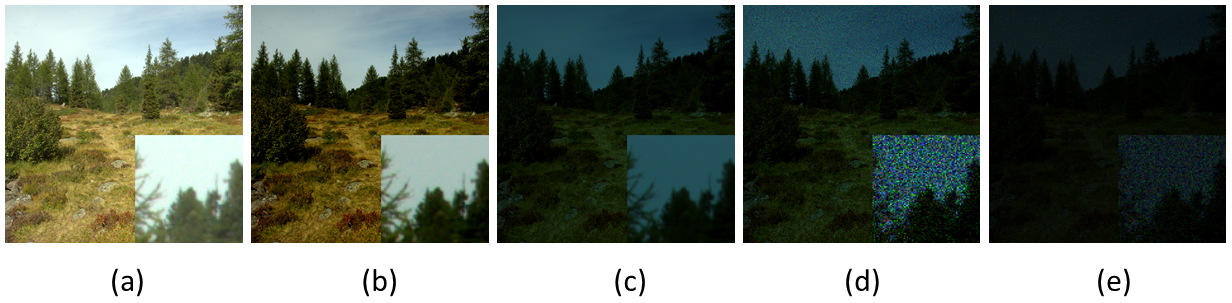
\includegraphics[scale=0.42]{simulation_all}
  \caption{An image after each step in our low-light simulation pipeline (a) Original Image (b) Black Level (c) Black Level + Color Distortion (d) Black Level + Color Distortion + Poisson Noise (e) Black Level + Color Distortion + Poisson Noise + Gamma Correction}
  \label{fig: simulation results}
\end{figure}

\subsection{Model Architecture}
Our model is built on the idea of how humans would try to observe information in dark images. If a human would want to observe information in a dark image, they would look very closely at a small portion of the image and distinguish between objects. This concept of viewing closely to understand the shapes and objects in a dark image is the intuition behind our model. We are able to capture this intuition using a deep Convolutional Neural Network whose architecture is illustrated in  Figure \ref{fig:model}.

Our simulated training data and SID data vary in size. Therefore, in order to train and test properly on each dataset, we extract patches of fixed size from each image. We only use one patch at a time during training. However, during testing, we evaluate our model on all patches generated from an image and then stitch them together. 

Our End-to-End model, shown in Figure \ref{fig:model}, is defined by (a) an initial Convolutional phase where max pooling decreases height and width by a factor of 2 at each of 4 Convolutional blocks while increasing channels by a factor of 2. The fifth Convolutional block consists of two Convolutional layers without a max pooling layer found in the previous 4 Convolutional blocks. The fifth Convolutional block serves as a transition point in our model. The next 4 Convolutional blocks, (b), use upsampling to reduce the number of channels by a factor of 2 at each block while also increasing height an width by a factor of 2. The final block (c) includes a Convolutional layer then a linear algebra transformation, in which values from the depth dimension are moved in spatial blocks to the height and width dimensions. This reduces the number of channels by a factor of 3 while doubling the height and width. The output dimensions of $64 \times 64 \times 3$ now match the input dimensions of $64 \times 6 \times 3$. We use $Y_{pred}$ and $Y_{true}$ to compute our $MAE$ loss function. This model architecture is based on that used by Chen et. al. (2018) \cite{chen2018learning}. 

\begin{figure}[ht]
  \centering
  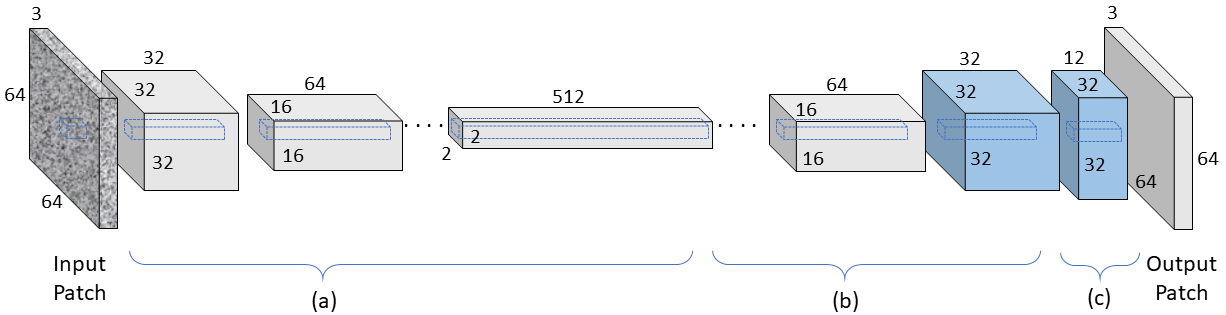
\includegraphics[scale=0.4]{model}
  \caption{A $32 \times 32 \times 3$ patch is taken from our input image patch of $64 \times 64 \times 3$. Part (a) consists of Convolutional blocks with a Max Pooling layer in each of 4 blocks. Block 5 is $2 \times 2 \times 512$ with only two Convolutional layers. Part (b) consists of 4 upsampling blocks which increase height and width while reducing the number of channels. Block 5 is converted from $2 \times 2 \times 512$ to $4 \times 4 \times 256$ in block 6. Part (c) uses a Convolutional layer of $32 \times 32 \times 12$ with a linear algebra transformation to output a tensor of $64 \times 64 \times 3$. The final two Convolutional blocks (highlighted in blue) are allowed to vary during the retraining phase of transfer learning.}
  \label{fig:model}
\end{figure}


\subsection{Model Tuning}

Our end-to-end CNN model is trying to solve 4 implicit subtasks - (a) Image with black level, (b) Image with black level, color distortion, (c) Image with black level, color distortion, Poisson noise, and (d) Image with black level, color distortion, Poisson noise, and gamma correction. This required us to break apart each subtask to assess the accuracy of our approach. Figure \ref{fig:losses_all_4} shows the validation loss on each subtask. The subtasks were defined using function compositions of image manipulations. Figure \ref{fig:losses_all_4} shows a reduction in validation loss decrease when epochs increase except for "Black Level, Color Distortion". Considering each subtask for fine-tuning, we were able to reduce loss after peaking by adjusting the learning rate. We analyzed learning rates from $[10^{-4}, 10^{-2}]$ and found $\alpha = 10^{-3}$ to have the best result. We also increased the number of layers from 5 layers to a deeper architecture with 27 layers and found a more favorable reduction in loss. We used only Convolutional and Max Pooling layers because Dense, or fully-connected, layers have more connections increased the training time and memory requirement. We were able to use a transformation of a convolutional block to achieve similar dimensionality to our $Y_{true}$ image. We optimize our model for Mean Absolute Error (MAE) loss using the Adam optimizer. 

Once we fine-tune our model for MAE, we evaluate our results using the Peak Signal-to-Noise Ratio (PSNR). This metric, calculated as a function of the Dark image, $D_{m\times n\times 3}$ and Bright image, $B_{m\times n\times 3}$ is defined as
\[
PSNR(D_{m\times n\times 3}, B_{m\times n\times 3}) = 20\cdot \log_{10}(\frac{255}{\sqrt{MSE(D_{m\times n\times 3}, B_{m\times n\times 3})}})
\]
where \(MSE\) refers to the Mean Squared Error. In this case, we find that PSNR is inversely related to our MAE loss: the higher the PSNR, the more signal our prediction has captured, and, thus, the better the prediction. We choose this evaluation metric because of its prevalence in the imaging community and also to compare the predictions of our model with the SID model in Table \ref{table:results_table}.

\begin{figure}[ht]
  \centering
  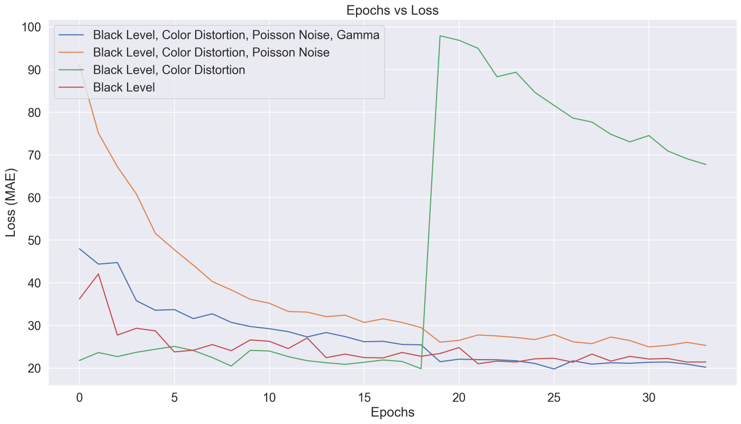
\includegraphics[scale=0.36]{losses_all_4}
  \caption{Sub-tasks of our end-to-end CNN model broken out by the function compositions which simulate various natural low-light image properties. "Black-Level, Color Distortion" is very sensitive to learning rate. The loss function, MAE, decreases as epochs increase for each image simulation sub-task. Each subtask was trained for 50 epochs.}
  \label{fig:losses_all_4}
\end{figure}

After choosing our hyperparameters and demonstrating the performance of each subtask for our end-to-end model, we trained our model on the simulated Raise dataset, in which the input images were transformed into low-light images using our simulation pipeline (Figure \ref{fig: simulation pipeline}). Training was done for 100 epochs, which took approximately 100 hours. 

Figure \ref{fig:simulated_prediction} shows us our model predictions for an image from the test set across the 100 trained epochs. We were able to generate these images by checkpointing at each epoch, restore a specific checkpoint, then predicting an image. It is most insteresting to see how, at first, the model learns to brighten the image while correcting the colors. We can see qualitatively that the quality of our prediction improves as our model trains for more epochs, but the remains black and white and gains color very slowly. Preliminary testing has suggested that additional training will help bring out the color and increased resolution in our predicted image.

\begin{center}
\begin{figure}[t!]
  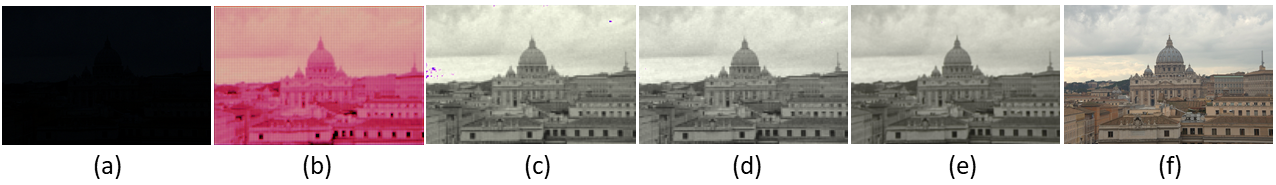
\includegraphics[scale=0.42]{simmulated_pred_each_epoch}
  \caption{End-to-End model prediction on image from test set of Raise data. We can observe image quality improve with more training epochs. (a) Input image, (b) after 1 epoch, (c) after 45 epochs (d) after 65 epochs, (e) after 100 epochs (final prediction), (f) True image.}
  \label{fig:simulated_prediction}
\end{figure}
\end{center}

\subsection{Transfer Learning}
After training our finalized deep CNN model on the simulated data, we transfer it to the real SID images. On such method is zero-shot learning, in which no additional training is performed and the model is tested on new data \cite{socher2013zeroshot}. Additionally, we perform transfer learning by freezing all but the last two blocks of layers from our model and retrain a fraction of the SID training data. In this sense, we only allow the weights of the last two blocks to vary. These are indicated as the blue blocks in Figure \ref{fig:model}. 

In order to emphasize the significance of our transfer learning approach, we only select 10\% of the training data for retraining. This means that, compared to the SID model, which was trained using 2000 bright-dark image pairs, we retrain our model on 200. Since only weights from the last two convolutional block were allowed to vary, this process converged relatively quickly: only 7 hours for 250 epochs. 

 \section{Experiment}

We evaluate our model based on the average PSNR of our testing data and performed a total of 4 tests. First, we evaluate the original model (prior to transfer) on the test set of the simulated images from RAISE 6k. Then, we evaluate our model via zero-shot learning on the test set of SID. Next, we evaluate, the transfer learning model on the test set of SID. Finally, we present the average PSNR from \textit{chen et. al. (2018)} \cite{chen2018learning}. Each resulting average PSNR on the test set, accompanied by its respective training set size and the number of epochs, is displayed in Table \ref{table:results_table}.

\begin{table}[ht]
    \centering
    \begin{tabular}{lllll}
    \toprule
          \multirow{3}{*}{} &  &No. Training&No. Epochs& \\
                           Model &Dataset& Images from &Initial / Transfer& PSNR\\
                            &  &Dataset&  &\\
      
    \midrule
    Ours & RAISE 6k & 6000  & 100\space\space\space\space/\space\space-  & 15.73 \\
    Ours & SID & 0 & 100\space\space\space\space/\space\space0  & 6.33 \\
    Ours& SID & 200 & 100\space\space\space\space/\space\space250 &10.19 \\
    SID Model& SID& 2000 & 4000\space\space/\space\space\space- &28.88\\
    \bottomrule
  \end{tabular}
  \\[10pt]
    \caption{Test results for our model on our test set of RAISE 6k images, zero-shot learning on the test set of SID images, transfer learning on test set of SID images, and results from \textit{chen et. al. (2018)} \cite{chen2018learning}. Our transfer model obtains comparable results with less than 10\% of the SID training data and 2.5\% initial epochs}
    \label{table:results_table}
\end{table}
Table \ref{table:results_table} shows that our model produces comparable results on the test set for Raise dataset, however, the PSNR drops when we perform a zero shot on the SID data. This is expected as our model does not learn device specific features. Our training is done on simulated data which helps it capture more general features of low light image enhancement. Once we perform transfer learning on the SID data for 250 epochs we see a significant increase in both the quantitative results (PSNR 10.19) and the qualitative result (Figure \ref{fig:final_predictions}(c)). This successfully shows the impact of transfer learning and the ability of our initial model to capture high level features. 

To show a qualitative comparison between our transfer learning model and the pre-trained SID model, we evaluate our model on a SID image pair using for zero shot, transfer, and the SID model. The resulting images are displayed in Figure \ref{fig:final_predictions}. 

\begin{figure}[t!]
  \centering
  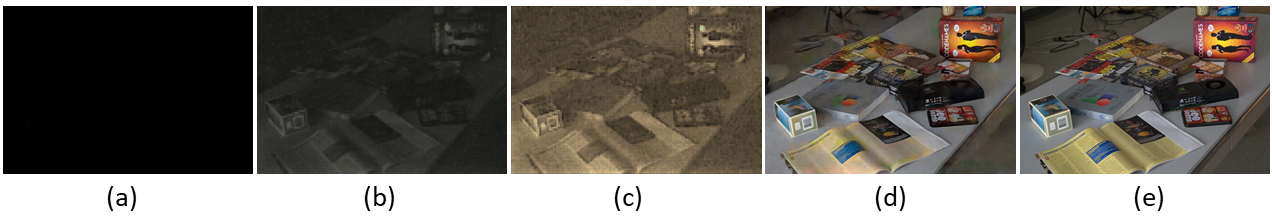
\includegraphics[scale=0.42]{Final_predictions}
  \caption{We can see predictions of our model for an image from the test set of SID data comapred to the result from \textit{Chen et. al. (2018)} \cite{chen2018learning} (a) Low light image, (b) Zero-Short prediction from our model, (c) Our model prediction after applying transfer learning on SID training data for 250 epochs, (d) Prediction from \textit{Chen et. al. (2018)} \cite{chen2018learning}, (e) Original Image}
  \label{fig:final_predictions}
\end{figure}

\section{Discussion}
Our analysis shows that a CNN for low-light image enhancement can be trained successfully on simulated images. It also shows that applying transfer learning on this model provides significant improvements for a particular device/domain (results on SID data). This transfer learning approach took only 10\% of the real world data as compared to \textit{Chen et. al.} \cite{chen2018learning}. We also presented a novel approach to simulate low-light images.

The two bottlenecks we faced with our model were computational resources and memory. This prevented us from storing the data on our local computers and drastically increased the cost of computing on AWS. Fortunately, we were granted access to MIT Lincoln Laboratory's server to train our models using a Tesla K80 and an Intel Xeon processor. Even so, we were only able to train our model for 100 epochs (100 hours) as compared to \textit{Chen et. al.}  who trained it 4000 epochs \cite{chen2018learning}. Due to this our model was not able to identify the colors in the image accurately. For our proof of concept for our model, initially, we trained our model on low-resolution CIFAR10 \footnote{https://www.cs.toronto.edu/~kriz/cifar.html}, where we observed a similar pattern. During the first 600-700 epochs, the image started getting sharper and denoised and once it reached a 1000 epochs, it started identifying color. Once we found that our model worked well on CIFAR10 images, we rebuilt it for higher resolution images. In this case, using RAISE-6k dataset, we were limited by memory and hence couldn't use larger patch sizes or variable sized images to train our model. 

In the future, we would like to try replacing our low-light simulation process with a neural network or a GAN, as currently, our simulation process cannot identify artificial light sources (such as street lamps, LED lights). These sources stay bright even in low light conditions. We would also like to run our model for a higher number of epochs to obtain comparable results to \textit{Chen et. al.} \cite{chen2018learning}. 

We are extremely grateful to \textbf{MIT Lincoln Labs} who agreed to provide us with a server for this project. Our images and code can be accessed at  \href{https://github.com/tbonza/CS7180}{"github.com/tbonza/CS7180"}.

%\newpage
\bibliographystyle{unsrt}
\bibliography{references}

\end{document}
